\subsubsection{Legge di Boltzmann e legge di Saha}
Cerchiamo adesso di capire da cosa dipende l'origine e l'intensità delle righe nello spettro di una stella. 

L'esistenza delle righe spettrali è regolata da due leggi: la legge di Boltzmann e la legge di Saha.

La legge di Boltzmann stabilisce come varia il rapporto delle popolazioni $N_a$ e $N_b$ di due livelli in base alla temperatura. Se con il pedice $a$ ci riferiamo al livello più alto energeticamente e con $b$ a quello più basso, l'equazione di Boltzmann sarà

\begin{equation}
  \frac{N_a}{N_b}=\frac{g_a}{g_b}e^{-\frac{(E_a - E_b)}{k_B T}}
  \label{eq:legge_di_Boltzmann}
\end{equation}

dove $g_a$ e $g_b$ sono i pesi statistici e $E_a - E_b$ è la differenza in energia tra i due livelli.

Tale equazione ci dice che il rapporto $N_a/N_b$ aumenta all'aumentare della temperatura (ciò è ovvio, perché con questa aumentano i processi collisionali e quindi il numero di elettroni negli stati eccitati). In particolare, per $T \to \infty$, il rapporto tra le due popolazioni tende al rapporto tra i pesi statistici $g_a/g_b$.

Il rapporto $N_a/N_b$ è piccolo se $E_a - E_b \gg k_B T$. In tal caso abbiamo elettroni disponibili ad assorbire fotoni della giusta lunghezza d'onda e quindi si avrà la riga spettrale.

\vspace{0.2cm}Un altro fattore collegato alla temperatura è la presenza o meno di atomi di ionizzati. Ad esempio, affinché esista la riga $H_{\alpha}$ deve esistere l'idrogeno neutro: non deve essere ionizzato. Sono quindi di nostro interesse le temperature che garantiscano una certa quantità di atomi di idrogeno neutri. (Abbiamo visto che laddove la temperatura aumenta raggiungendo le decine di migliaia di gradi, l'idrogeno si ionizza totalmente). Quindi, la presenza o meno dell'idrogeno neutro dipende dalla temperatura secondo la relazione:

\begin{equation}
  \frac{N_{i+1}}{N_i}=\frac{2 Z_{i+1}}{n_e Z_i} \left( \frac{2 \pi m_e k_B T}{h^2} \right)^{\frac{3}{2}} e^{-\frac{\chi_i}{k_B T}}
\end{equation}

dove $\chi_i$ è l'energia di ionizzazione necessaria a portare l'elettrone dallo stato $i$ a quello $i+1$, $n_e$ è la densità del numero di elettroni liberi e $Z$ è la funzione di partizione, una somma pesata dei modi in cui l'atomo o lo ione può distribuire i suoi elettroni nei suoi livelli energetici.

Essa prende il nome di legge di Saha, la quale ci dice che la temperatura non deve essere troppo elevata.

D'altro canto però la temperatura non deve essere nemmeno troppo bassa, per garantire il popolamento dei livelli più alti. Il compromesso per l'esistenza di una riga nasce quindi dal prodotto tra la probabilità che il livello sia ionizzato e quella che sia popolato. Noi dobbiamo sostanzialmente fare il prodotto di una funzione che all'aumentare della temperatura aumenta lo stato di ionizzazione: ad esempio l'idrogeno a $85000$ K è tutto ionizzato; di conseguenza una stella che presenti una temperatura T pari a $85000$ K non potrà presentare righe dell'idrogeno perché esso sarà ivi scomposto in protoni ed elettroni. Di contro abbiamo bisogno che il livello sia popolato.

\begin{figure}[H]
  \centering
  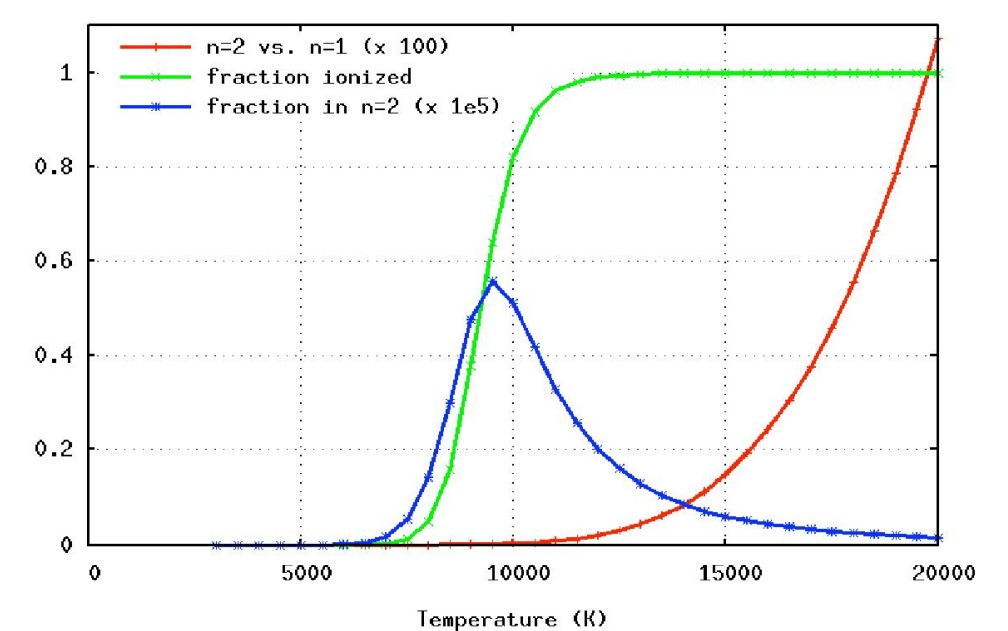
\includegraphics[width=10cm]{Saha.jpg}
  %\caption{Atomi di idrogeno in una atmosfera stellare}
  \label{fig:Boltzmann*Saha }
\end{figure}

Nel grafico la linea rossa rappresenta la percentuale di atomi in cui gli elettroni si trovano nello stato più alto rispetto a quello più basso; la linea verde rappresenta la frazione di atomi ionizzati; infine la linea blu rappresenta la frazione di atomi in cui l'elettrone è nel livello superiore. Pensiamo ad esempio al secondo livello dell'atomo di idrogeno: a temperatura bassa gli elettroni sono tutti nel livello inferiore; se la temperatura aumenta il livello si popola e se essa continua a crescere nel tempo, il livello si ionizza e l'atomo decade; c'è una temperatura in cui ogni livello risulta al massimo della popolazione e dipende, attraverso la ionizzazione, dalla densità elettronica.

Ciò che noi osserviamo è un andamento di questo genere tra la popolazione di un livello e la depopolazione dello stesso per ionizzazione. Nel caso dell'atomo di idrogeno il picco si osserva per T=10000 K; ci aspettiamo quindi che le stelle nel cui spettro le righe dell'idrogeno sono al massimo della loro intensità siano caratterizzate da questa temperatura.

Andamenti di questo genere possono essere costruiti per tutti gli elementi, non solo per l'idrogeno:

\begin{figure}[H]
\centering
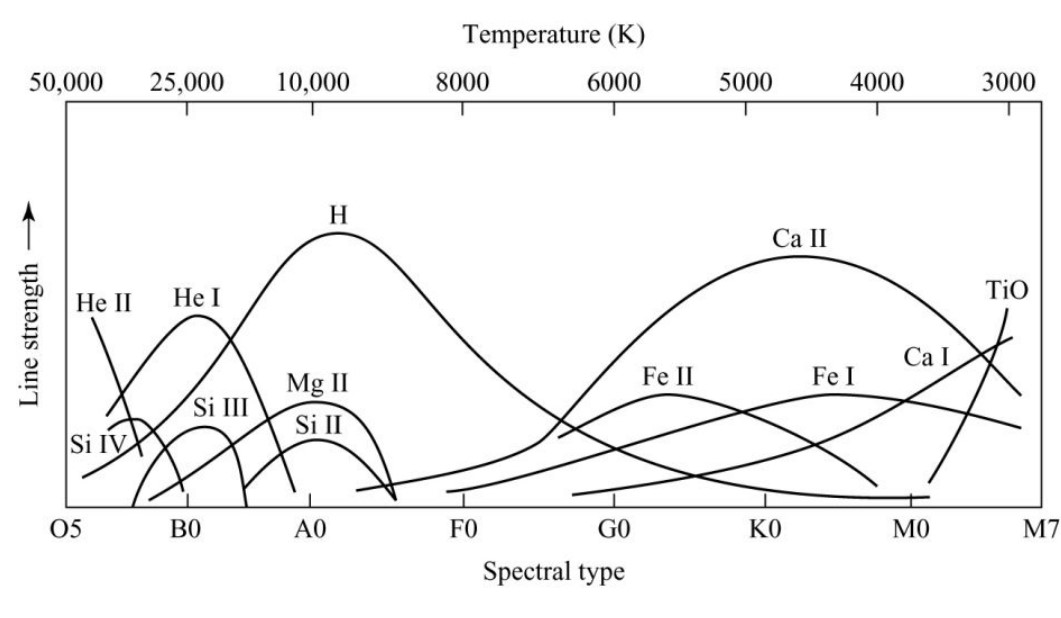
\includegraphics[width=10cm]{173507.jpg}
\end{figure}

Nota: in astrofisica, dato un elemento con stato di ionizzazione $n$ esso si indica con il numero $n+1$ scritto in cifre romane: ad esempio il Ferro neutro si indica con "Fe I", il ferro una volta ionizzato con "Fe II" e così via.

Osservando il grafico si possono fare alcune osservazioni: mentre l'idrogeno, che ionizza a 13.6 eV, ha un massimo in corrispondenza di T=10000 K, il calcio ionizza a temperature molto più basse, tant'è che in corrispondenza di T=5000 K è già ionizzato una volta. Quindi in un'atmosfera caratterizzata dalla presenza di tali atomi, la loro abbondanza varia in funzione della temperatura.

Avendo osservato che le righe spettrali (a parità di abbondanza degli elementi) cambiano in funzione della temperatura, si può pensare di attribuire alle stelle una temperatura sulla base dei loro spettri. Gli spettri potrebbero quindi essere ordinati in base all'intensità delle loro righe spettrali.

\begin{figure}[H]
  \centering
  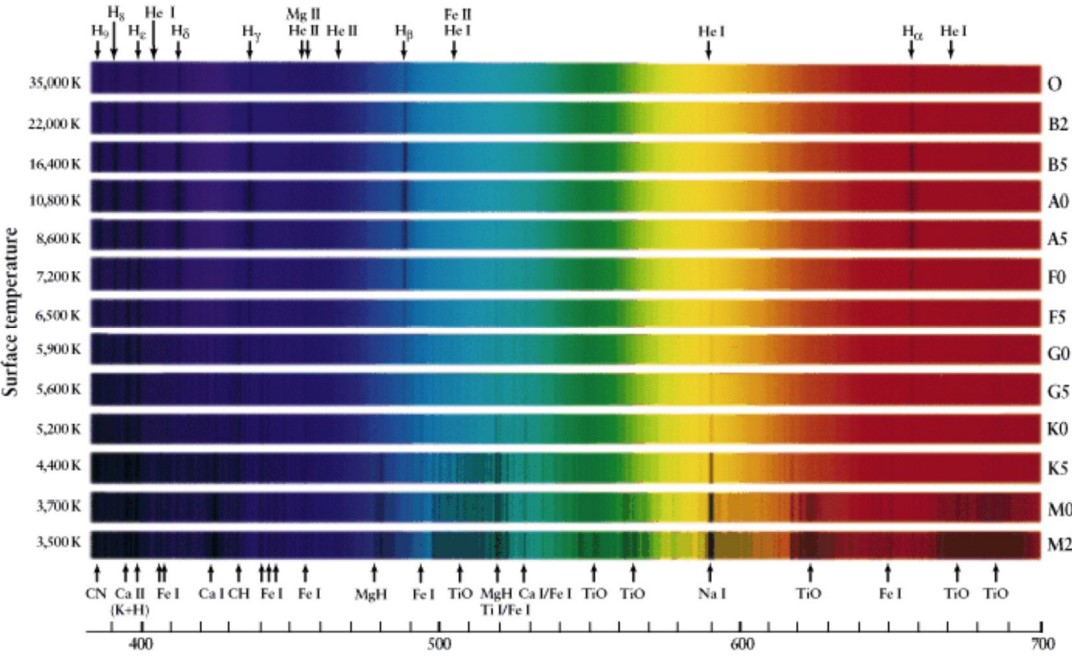
\includegraphics[width=10cm]{174642.jpg}
\end{figure}

Le stelle possiedono quindi una temperatura compresa tra 3500 K e 35000 K. Ogni serie di righe spettrali diventa così un marker di temperatura. Se osserviamo le righe spettrali come una sorgente di opacità (del resto sottraggono radiazione), mentre l'opacità degli atomi è comune da osservare, quella degli ioni negativi viene osservata a temperature molto basse in quanto caratterizzati da un'energia di legame prossima allo zero, ionizzandosi in presenza di fotoni dell'ordine dei $\mu$m.

\subsubsection{Coefficienti di Einistein}

Se è vero che le righe spettrali sono dovute alle transizioni legato-legato (dell'idrogeno), perché queste assumono intensità diversa negli spettri?

La prima risposta potrebbe essere l'abbondanza di idrogeno\footnote{N.B.\,: Il numero di fotoni non incide sul coefficiente di estinzione perché l'estinzione è relativa, è una percentuale di ciò che attraversa la materia. Occorre quindi considerare la variazione di luminosità e non la stessa in termini assoluti.}, ma all'interno di un atomo la probabilità di passare da un livello all'altro non è detto sia uguale. Vedremo che tale probabilità è espressa dai \textbf{coefficienti di Einstein}.

\footnote{Anche questo paragrafo è preso dall'Innocenti, lol.}I coefficienti di Einstein sono dei coefficienti legati alla probabilità per unità di tempo che avvenga un certo fenomeno. Furono introdotti dal celebre fisico tedesco attraverso un ragionamento fisico di questo tipo: consideriamo due livelli energetici di un sistema atomico e indichiamo con $\epsilon_a$ e $\epsilon_b$ le energie dei livelli superiore e inferiore, rispettivamente, e con $g_a$ e $g_b$ le relative degenerazioni. Sia poi $\nu_{ab}$ la frequenza della transizione fra i due livelli, con

\begin{equation*}
  h \nu_{ab}=\epsilon_a - \epsilon_b
\end{equation*}

Se il sistema atomico si trova immerso in un campo di radiazione avente, alla frequenza $\nu_{ab}$, intensità media $J_{\nu_{ab}}$, allora si ha una probabilità di transizione per unità di tempo dal livello inferiore a quello superiore data

\begin{equation*}
  \pi_{ba}=B_{ba} J_{\nu_{ab}}
\end{equation*}

Questa espressione è conforme all'esperienza in quanto essa prevede, essendo per ipotesi $B_{ba}$ indipendente dal campo di radiazione, che la probabilità di transizione sia proporzionale all'intensità media del campo di radiazione, una legge che corrisponde al ben noto fenomeno dell'assorbimento. D'altra parte,
per la probabilità di transizione dal livello superiore a quello inferiore, le leggi fisiche (note al momento del lavoro di Einstein) portavano semplicemente a un'equazione del tipo

\begin{equation*}
  \pi_{ab}=A_{ab}
\end{equation*}

con $A_{ab}$ indipendente dal campo di radiazione. Infatti, al momento, era noto soltanto il fenomeno dell'emissione spontanea e non quello dell'emissione stimolata\footnote{L'emissione stimolata è un processo quantistico che può verificarsi in un sistema atomico o molecolare quando gli atomi o le molecole vengono eccitati da radiazione elettromagnetica. Questo fenomeno è alla base del funzionamento dei laser. Esso si verifica quando un atomo o una molecola già in uno stato eccitato viene colpito da un fotone con un'energia corrispondente alla differenza di energia tra lo stato eccitato e uno stato di energia inferiore. In risposta, l'atomo o la molecola emette un secondo fotone identico a quello incidente, creando due fotoni coerenti in termini di fase e direzione.}.

Einstein osservò che le due espressioni per $\pi_{ba}$ e $\pi_{ab}$ erano incompatibili con le leggi della termodinamica. Se si suppone infatti che il sistema atomico si trovi in una cavità all'equilibrio termodinamico alla temperatura $T$, siccome i coefficienti $A_{ab}$ e $B_{ba}$ sono indipendenti dal campo di radiazione, si ottiene che al limite per $\rm T \to \infty$ il rapporto $\pi_{ba}/\pi_{ab}$ tende anch'esso all'infinito, col risultato che tutti gli atomi verrebbero a trovarsi nel livello superiore, in palese contraddizione con quanto specificato dalla legge di Boltzmann che invece prevede un rapporto di popolazioni uguale al rapporto dei pesi statistici:

\begin{equation*}
  \frac{N_a}{N_b}=\frac{g_a}{g_b} e^{-\frac{\epsilon_a - \epsilon_b}{k_B T}}
\end{equation*}

Per risolvere questa contraddizione, Einstein postulò allora che nell'equazione per la probabilità di transizione $\pi_{ab}$ si dovesse aggiungere un nuovo termine, anch'esso proporzionale al campo di radiazione così da ottenere

\begin{equation*}
  \pi_{ab}=A_{ab} + B_{ab} J_{\nu_{ab}}
\end{equation*}

Con un semplice ragionamento termodinamico Einstein riuscì quindi a prevedere l'esistenza dell'emissione stimolata, un meccanismo fisico che non era noto al momento.

Sempre in base a considerazioni termodinamiche è poi possibile determinare le relazioni esistenti fra i vari coefficienti introdotti. In base alle equazioni precedenti la popolazione del livello superiore, $N_a$, obbedisce all'equazione differenziale

\begin{equation*}
  \frac{dN_a}{dt}=-(A_{ab} + B_{ab}J_{\nu_{ab}})N_a + B_{ba}J_{\nu_{ab}}N_b
\end{equation*}

In situazioni stazionarie (quindi $\frac{dN_a}{dt}=0$) si ottiene allora

\begin{equation*}
  \frac{N_a}{N_b}=\frac{B_{ba} J_{\nu_{ab}}}{A_{ab} + B_{ab}J_{\nu_{ab}}}
\end{equation*}

Supponendo di essere all'equilibrio termodinamico, e facendo il limite $\rm T \to \infty$ dell'equazione di Boltzmann, si ottiene

$$\lim_{T \to \infty} \frac{N_a}{N_b}=\frac{g_a}{g_b}$$

da cui segue che

$$B_{ba}=\frac{g_a}{g_b} B_{ab}$$

In generale, per $T$ arbitrario, sostituendo per $N_a/N_b$ il valore dato dall'equazione di Boltzmann, esprimendo $B_{ba}$ in termini di $B_{ab}$ e ricordando che all'equilibrio termodinamico l'intensità media del campo di radiazione è data dalla funzione di Planck ($J_{\nu_{ab}}=B_{\nu_{ab}}(T)$), si
ottiene, con un alcuni passaggi algebrici

$$A_{ab}=\frac{2h \nu_{ab}^3}{c^2} B_{ab}$$

Con questo ragionamento termodinamico si arriva quindi a stabilire la corretta
relazione fra i coefficienti di Einstein.

\vspace{0.2cm}Introdotte queste notazioni, siamo adesso in grado di scrivere le equazioni dell'equilibrio statistico per un atomo con un numero arbitrario di livelli energetici. Per la popolazione di un generico livello $n$, indicando con l'indice $i$ i livelli inferiori (cioè aventi energia minore) e con l'indice $s$ i livelli superiori (cioè aventi energia maggiore), l'equazione di evoluzione della popolazione si scrive

\begin{eqnarray}
  \begin{split}
    \frac{dN_n}{dt}&=\sum_{i}B_{in}J_{{\nu}_{ni}}N_i + \sum_{s}A_{sn}N_s + \sum_{s}B_{sn}J_{{\nu}_{ns}}N_s\\
    & - \sum_{i}A_{Ni}N_n - \sum_{i}B_{in}J_{{\nu}_{ni}}N_n - \sum_{s} B_{ns} J_{\nu_{sn}} N_n
  \end{split}
  \label{eq:coeff_einstein}
\end{eqnarray}

\begin{figure}[H]
  \centering
  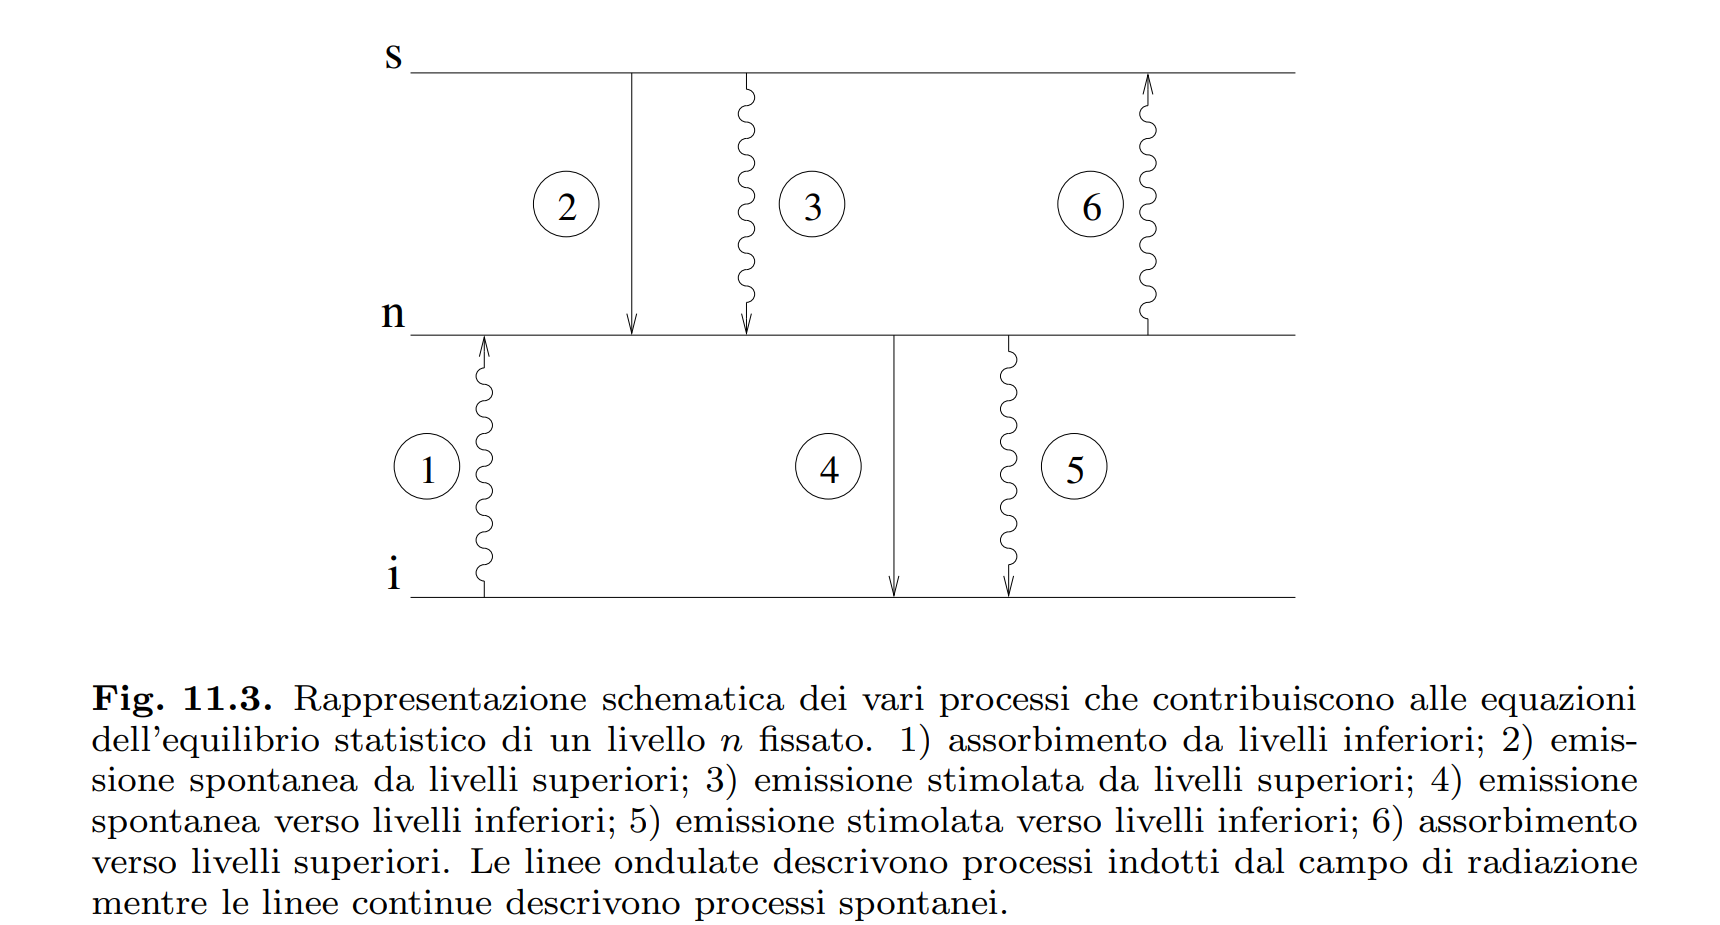
\includegraphics[width=0.9\textwidth]{immagini/processi_popolazione_livello_n.png}
\end{figure}

I sei termini che compaiono nell'equazione precedente sono rappresentati schematicamente nella figura appena sopra, nella quale le linee continue rappresentano transizioni spontanee (proporzionali ai coefficienti di Einstein $A$) mentre quelle ondulate rappresentano transizioni indotte dal campo di radiazione (proporzionali ai prodotti di coefficienti di Einstein $B$ per l'intensità media del campo di radiazione $J$). In particolare, le linee ondulate che terminano con una freccia diretta verso l'alto rappresentano fenomeni di assorbimento, mentre quelle che terminano con una freccia diretta verso il basso rappresentano fenomeni di emissione stimolata. I numeri riprodotti entro i cerchi nella figura sono in connessione con l'ordine dei vari termini dell'Eq. \eqref{eq:coeff_einstein}. In altre parole, i termini 1 e 6 rappresentano processi di assorbimento prodotti dal campo di radiazione; quelli 2 e 4 rappresentano processi di emissione spontanea; infine, i termini 3 e 5 rappresentano processi di emissione indotta o stimolata. Si noti che i processi 1, 2, e 3 contribuiscono a popolare il livello $n$ e sono preceduti nell'equazione da un segno più, mentre i processi 4, 5, e 6 contribuiscono a depopolarlo e sono preceduti da un segno meno.




\subsubsection{Classificazione degli spettri stellari in astronomia classica}

Padre Angelo Secchi fu il primo a classificare spettri stellari, attribuendo loro delle lettere dell'alfabeto.

\begin{figure}[H]
  \centering
  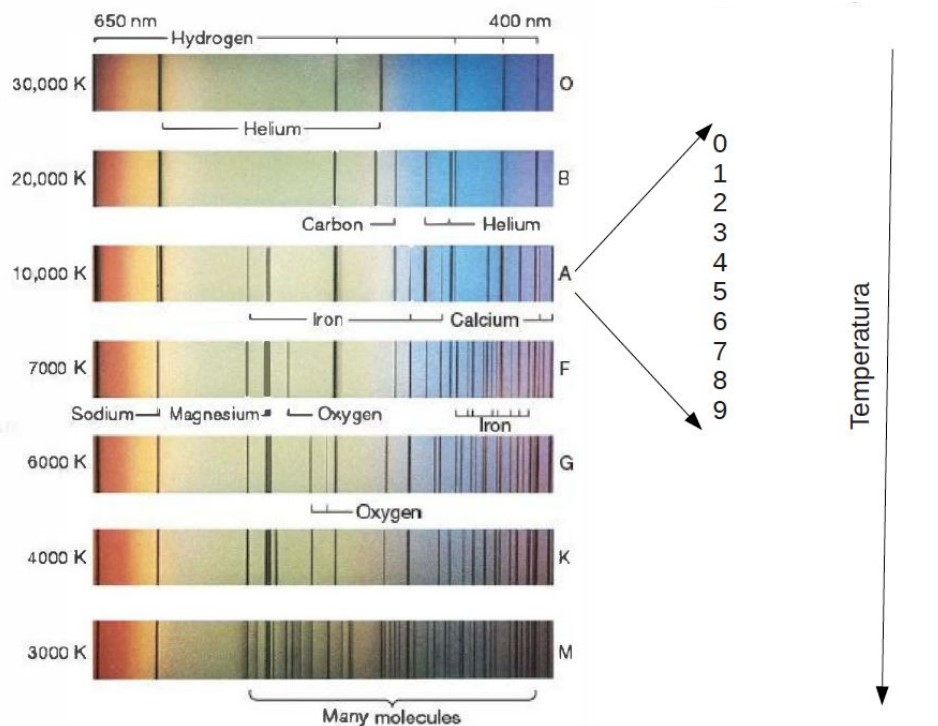
\includegraphics[width=10cm]{angelo_secchi.jpg}
\end{figure}

Egli credeva che quelle con la grande banda nera al centro fossero le più belle e le indicò con la lettera A, e così via. Questa nomenclatura è in vigore ancora oggi, anche se alcune delle lettere introdotte da Angelo Secchi vennero escluse nei casi in cui non erano state osservate stelle ma mezzi interstellari, i quali in realtà assorbono fotoni dalle stelle realizzando delle bande che possono essere anche più intense. Gli spettri identificati da lettere dell'alfabeto sono poi stati riordinati in funzione della temperatura: ad esempio, le stelle più calde sono quelle che Secchi identificò con la lettera "O", seguite da "B", "A", "F", "G", "K" e "M"\footnote{Un modo utilizzato dagli astronomi per ricordare la sequenza delle classi spettrali è la frase inglese "Oh Be A Fine Girl/Guy, Kiss Me".}. Ancora oggi, quando si parla di stelle, si fa riferimento alla lettera con cui vengono identificate e che prende il nome di "tipo spettrale". Il nome dell'elemento riportato sotto lo spettro è quello che dà origine alle righe più intense; in ordine, le "O" sono le righe dell'elio ionizzato, le "B" dell'elio neutro, le "A" dell'idrogeno  le "F" del calcio e così via.

Oggi che siamo in grado di vedere spettri di oggetti molto piccoli e freddi (l'emissività totale ha un andamento che va come ${\sigma}T^4$) che sappiamo essere dominati non da atomi ma da bande molecolari. Le stelle più fredde sono quindi caratterizzate da bande di metano, ossido di titanio, ossido di vanadio: si tratta di una classificazione più recente rispetto a quella classica, che terminava con la lettera M, cui si sono aggiunte le lettere L e T.

A conclusione di ciò chiariamo che l'intensità delle righe non dipende dall'abbondanza bensì dalla condizione fisica dell'atmosfera. Se si tiene conto di ciò, tutte le stelle nei dintorni hanno la medesima composizione chimica; estraendo il contributo della temperatura alla riga, risulta che l'idrogeno è uguale in tutte le stelle (almeno le più vicine).

La classificazione di Secchi risultò presto troppo grossolana, in seguito all'aumento della precisione degli strumenti di misura adoperati; questo è il motivo per cui ogni tipo spettrale viene a sua volta suddiviso in 10 (ad esempio la A-0 è la più calda delle stelle A, la più fredda è una A-9).



Ricapitolando, sulla base della presenza e dell'intensità delle righe spettrali dei vari elementi è stata stabilita una classificazione spettrale delle stelle, in particolare sono ordinate per temperature decrescenti. La classificazione avviene con una lettera, ad esempio le stelle di tipo spettrale “O” sono le più calde e sono caratterizzate dalla presenza di He ionizzato; a seguire abbiamo le stelle “B” caratterizzate dall'intensità massima della riga di He neutro; poi le stelle “A” caratterizzate dall'H e Ca ionizzato.

Inoltre, sulla base della distribuzione spettrale delle stelle e l'utilizzo di filtri fotometrici, cioè strumenti in grado di selezionare porzioni di spettro, abbiamo definito l'indice di colore

$$B-V=m_B-m_V=2.5\log_{10}{\frac{F_B}{F_V}}$$

cioè il rapporto dei flussi in due bande diverse dello spettro, che definisce la pendenza di uno spettro. Associando ad ogni colore ad una temperatura si è costruito il diagramma di Hertzsprung-Russel, in cui le stelle sono raggruppate in sequenze.



%Gli astronomi, piuttosto che le aree, preferiscono misurare questa quantità \textbf{MA QUALE} perché la definizione di larghezza equivalente non ha unità di flusso, quindi non prevede una calibrazione assoluta degli strumenti, ma soltanto una calibrazione relativa: 





%esaminiamo infine il fenomeno delle microturbolenze, che possiamo immaginare come delle "bolle", blocchi di molecole\footnote{\E chiaro che in un plasma non si può parlare di molecole: la materia è ionizzata, ma il concetto è uguale.} che si muovono insieme (posso dire all'unisono?). Queste bolle possono essere ferme o in moto




\vspace{0.2cm}Abbiamo visto come una riga spettrale si formi in condizioni ben precise di temperatura e come questo possa portare ad una classificazione delle stelle sulla base della presenza di righe (perché a queste, in pratica, corrisponde una temperatura). Il range di temperatura molto limitato è dovuto a due fenomeni: la ionizzazione e la popolazione degli atomi. Abbiamo anche visto che, dato che gli assorbitori si muovono, le righe spettrali portano con loro informazioni sulla dinamica dell'ambiente. Ad esempio, si osserva un allargamento della riga dovuto all'effetto Doppler, indotto dall'agitazione termica. Questa è un'ulteriore conferma del concetto di temperatura che stabilisce quali livelli sono popolati. Ricordiamo infatti che quando un sistema è in equilibrio termodinamico, cioè quando non si hanno variazioni su grande scala, tutte le quantità devono essere esprimibili in funzione di una sola grandezza che è la temperatura.

\subsubsection{Dipendenza dell'intensità delle righe spettrali dalle condizioni del plasma}
Fino ad ora abbiamo visto la forma che avrebbe una riga spettrale, ma non abbiamo detto se una riga spettrale si forma o meno. Abbiamo anche visto quali sono le condizioni affinché si formi una riga, ad esempio i livelli devono essere occupati. Ma quando si forma effettivamente una riga spettrale?

Per rispondere a questa domanda dovremmo risolvere l'equazione del trasporto radiativo, perché i processi che avvengono sono due: emissione e assorbimento. Serve quindi un bilancio tra quelli che sono i processi di assorbimento, rappresentati dal coefficiente di estinzione, e quelli di emissione. Il problema ora sta nel trovare la forma del coefficiente di emissione.

Per iniziare, immaginiamo di essere in una condizione di equilibrio termodinamico, cioè di trovarci in un volume $dV$ in cui tutti i processi (termici, meccanici, chimici, radiativi) siano in equilibrio\footnote{Questo equivale a dire che se esiste un qualunque processo, deve esistere il processo opposto (es. se un oggetto si avvicina un altro si allontana, è un equilibrio dinamico).}. In questa condizione si potrebbe dire che i processi di assorbimento sono eguagliati da quelli di emissione, cioè

$$\chi_\nu I_\nu \, dV \, d\Omega \, d\nu \, dt
=\eta_\nu \, dV \, d\Omega \, d\nu \, dt$$

Consideriamo un atomo con l'elettrone nel livello più alto: dopo un po' di tempo, naturalmente, questo elettrone cadrebbe al livello più basso, emettendo un fotone che potrebbe lasciare l'ambiente e quindi non essere riassorbito con il conseguente raffreddamento dell'ambiente. Possiamo pensare, quindi, che le condizioni affinché ci sia equilibrio termodinamico siano che

\begin{enumerate}
  \item La maggior parte degli elettroni scende di livello non per emissione ma per collisione;
  \item Il libero cammino medio del fotone deve essere piccolo, in quanto vogliamo che esso non debba uscire dal volume (se se ne andasse si avrebbe una perdita di energia).
\end{enumerate}

Quindi, l'equilibrio termodinamico sostanzialmente richiede di avere collisioni capaci di riportare gli atomi nel livello più basso e che i fotoni non debbano uscire. Se queste condizioni sono verificate, il volume non avrà una variazione di intensità specifica, che quindi sarà uguale al rapporto tra emissione e assorbimento, che nell'equazione del trasporto radiativo abbiamo definito come funzione sorgente $S_\nu$:

$$I_\nu=\frac{\eta_\nu}{\chi_\nu}=S_\nu$$

Questo vuol dire che lo spettro di emissione del volume, dato che siamo all'equilibrio\footnote{Un esempio potrebbe essere la cavità con una piccola apertura considerata nella trattazione del corpo nero, dove i fotoni non possono uscire perché vengono assorbiti o riflessi dalla parete.}, è caratterizzato da un solo parametro che è la temperatura. Di conseguenza, la funzione sorgente sarebbe, di fatto, la funzione di Plank $B_\nu (T)$ ad una temperatura che è quella di equilibrio.

Queste condizioni si possono verificare anche in un ambiente non chiuso, nel caso in cui la variazione della lunghezza scala della temperatura sia molto più grande del libero cammino medio delle particelle (quindi le particelle non lasciano l'ambiente: collidono, partecipando al riempimento e svuotamento dei livelli energetici degli atomi, e se ci sono dei fotoni prodotti questi vengono riassorbiti in uno spazio molto più piccolo del volume considerato). In questo caso l'ambiente si trova in equilibrio termodinamico locale\footnote{Ovviamente non si hanno ambienti perfettamente in equilibrio termico locale, ma alcuni possono essere approssimabili a tali.} (LTE). Si tratta di una condizione favorevole, in quanto in questo modo è possibile conoscere la funzione sorgente e, di conseguenza conoscere il coefficiente di emissione, in quanto sarebbe quello di un corpo nero con un dato valore di temperatura.

\begin{minipage}{0.395\textwidth}
  \begin{figure}[H]
    \centering
    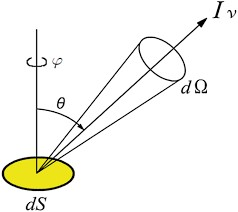
\includegraphics[width=5cm]{rappresentazione.jpg}
  \end{figure}
\end{minipage}
\begin{minipage}{0.6\textwidth}
  Per fare un passo avanti abbiamo bisogno di definire alcune quantità. Abbiamo già definito l'intensità specifica come la funzione che rappresenta la variazione di energia di una radiazione che attraversa una superficie $dS$ in una certa direzione proiettata $\theta$ all'interno di un angolo solido $d\Omega$ nell'unità di tempo e per unità di frequenza 
  $$dE_\nu=I_\nu(\theta,\Phi)d\nu (\cos\theta dS) d\Omega dt$$
\end{minipage}

\vspace{0.2cm}\E utile definire l'intensità totale, definita come l'integrale su tutte le frequenze dell'intensità specifica

$$I=\int I_\nu d\nu$$

Può essere utile anche chiedersi quanta intensità specifica ha attraversato la superficie dS in tutto l'angolo solido, quantità che viene definita \textit{intensità media}

$$J_\nu = \frac{1}{4\pi}\int I_\nu \, d\Omega$$

In alcuni processi, tuttavia, risulta più comodo fare riferimento alla densità dei fotoni (ad esempio per una transizione da un livello $a$ ad un livello $b$). Se

$$F_\nu=\oint I_\nu \cos\theta \, d\Omega$$

è il flusso della radiazione che attraversa la superficie $dS$, e la densità dei fotoni che hanno attraversato tale superficie è $\frac{I_\nu}{h\nu}$, allora il numero di fotoni che hanno attraversato $dS$ sarà

$$n_\nu = \oint \frac{I_\nu}{h\nu} \cos\theta \, d\Omega= \frac{4\pi}{c}\frac{J_\nu}{h\nu}$$

\textbf{guarda spettroscopia sezione 13.2}

Per cercare di capire cosa dà effettivamente origine ad una riga spettrale, consideriamo il caso più semplice (che non esiste) dell'atomo con due livelli energetici $E_a$ ed $E_b$, con $E_a > E_b$, ognuno con una sua probabilità di essere popolato e quindi una degenerazione $g$ (il numero di elettroni che possiamo allocare in quel livello). Ci possiamo chiedere quanti sono gli atomi che hanno l'elettrone nel livello $b$ e quanti quelli che hanno l'elettrone nel livello $a$. La probabilità di avere un depopolamento del livello $a$ è data dal numero $N_a$ di atomi che hanno l'elettrone nel livello $a$, moltiplicato per un coefficiente di decadimento naturale $A_{ab}$ per cui il livello si svuota, che viene normalmente definito come coefficiente di Einstein di emissione spontanea. Esiste, inoltre, la possibilità che l'elettrone passi dal livello $a$ al livello $b$ perché stimolato dalla radiazione ed è quindi possibile definire un coefficiente di Einstein $B_{ab}$ per emissione stimolata. La probabilità di quest'ultimo processo è legata ad $N_a$ e al campo medio di radiazione $J_{\nu_{ab}}$, e quindi all'intensità media. Infine, oltre a depopolarsi, il livello si può anche popolare per effetto di collisioni ed è quindi possibile definire un coefficiente di Einstein $B_{ba}$ per l'assorbimento. In definitiva

$$\frac{dN_a}{dt}= -A_{ab} N_a - B_{ab} J_{\nu_{ab}}N_a + B_{ba} J_{\nu_{ab}}N_b$$

Un ragionamento analogo può essere fatto per il livello $b$.

Questo ragionamento riguarda i processi legati al campo di radiazione e all'emissione stimolata, tuttavia, c'è anche la probabilità che un livello si popoli per effetto di collisioni. Queste ultime possono portare l'elettrone dal livello $a$ al livello $b$ e si chiamano collisioni super-elastiche con coefficiente $C_{ab}^S$, oppure portare dal livello $b$ al livello $a$, che vengono chiamate collisioni anelastiche con coefficiente $C_{ba}^A$.

Quando si parla di collisioni è importante che il coefficiente di collisione, che indica la probabilità di popolare un livello, sia legato al numero di collisioni. Notiamo inoltre che gli elettroni hanno una massa molto più piccola di quella degli atomi e di conseguenza si muovono con una velocità circa 2000 volte più grande di quella degli atomi, quindi normalmente quando si fa questo genere di calcolo si considera semplicemente la densità degli elettroni $N_e$. Si ha che

$$C_{ba}^A=N_e \int_{v_0}^{\infty}\sigma_{ba}(v)f(v)vdv$$

dove $\sigma_{ba}(v)$ è la sezione d'urto per un'eccitazione data da collisione per una velocità $v$, $f(v)$ è la distribuzione delle velocità degli elettroni e $v_0$ è la velocità minima per eccitare l'atomo dal livello $b$ al livello $a$. \E molto importante, quindi, conoscere con che velocità si stanno muovendo gli elettroni, la quale normalmente è legata alla temperatura. In maniera analoga si ha che 

$$C_{ab}^S=N_e\int_{0}^{\infty}\sigma_{ab}(v)f(v)v\,dv$$

dove $\sigma_{ab}(v)$ è la sezione d'urto per diseccitazione collisionale per una velocità $v$.

Tenendo conto sia dei processi collisionali che dei processi radiativi , l'equazione dell'equilibrio statistico per la popolazione del livello superiore risulta

$$\frac{dN_a}{dt}=-N_a (A_{ab} + B_{ab}J_\nu + C_{ab}^S)+ N_b(B_{ba}J_\nu + C_{ba}^A)$$

In condizioni stazionarie $\displaystyle \frac{dN_a}{dt}=0$, quindi il rapporto tra i numeri di atomi che hanno l'elettrone nel livello $a$ e quelli che lo hanno nel livello $b$ è pari a

$$\frac{N_b}{N_a}=\frac{A_{ab}+B_{ab}J_\nu +C_{ab}^S}{B_{ba}J_\nu+C_{ba}^A}$$

dove le uniche grandezze che entrano in gioco sono il campo di radiazione e i coefficienti di collisione.

\hrulefill

Svolgiamo alcuni \textsc{calcoli astromeccanici} per spiegare come si arriva al risultato che verrà enunciato subito dopo.

\vspace{0.2cm}$\bullet$ \textbf{Relazioni di Milne-Einstein}

\vspace{0.2cm}Quando la distribuzione di velocità degli elettroni collidenti è Maxwelliana, si può dimostrare, attraverso un ragionamento termodinamico, che i coefficienti collisionali introdotti sono collegati tra loro da una semplice relazione. Tale ragionamento termodinamico, dovuto a Milne, è molto simile a quello precedentemente sviluppato da Einstein per determinare le relazioni esistenti fra i coefficienti che intervengono nelle equazioni dell'equilibrio statistico per l'interazione atomo-radiazione (coefficienti di Einstein). Per questa ragione le relazioni che si ottengono sono dette relazioni di Milne o di Milne-Einstein.

Si consideri un atomo composto da due soli livelli, $a$ e $b$, soggetto a collisioni da parte di un plasma di elettroni aventi densità $N_e$. Se il sistema è in equilibrio termodinamico alla temperatura $T$, possiamo invocare il cosiddetto principio del bilancio dettagliato per asserire che il numero di transizioni collisionali (dovute agli elettroni) che avvengono fra il livello $a$ e il livello $b$ è esattamente bilanciato dal numero di transizioni collisionali (anch'esse dovute agli elettroni) che avvengono fra il livello $b$ e il livello $a$. In altre parole, all'equilibrio termodinamico la condizione di equilibrio deve valere per qualsiasi processo che contribuisca a popolare o depopolare i livelli atomici indipendentemente dal numero e dalle caratteristiche fisiche dei processi che sono simultaneamente in operazione (processi radiativi, processi collisionali sempre con elettroni, ma fra altre coppie di livelli, processi collisionali con altre specie atomiche, ecc.). In caso contrario, infatti, sarebbe possibile costruire una macchina ideale, lavorante in ciclo, che potrebbe produrre lavoro a spese di un'unica sorgente, il che contraddirebbe il secondo principio della termodinamica. Se indichiamo quindi con $\tilde{N}_a$ e $\tilde{N}_b$ le popolazioni dei livelli $a$ e $b$ all'equilibrio termodinamico, si deve avere, scrivendo l'equazione di evoluzione per la popolazione del livello $a$,

\begin{equation*}
  0=\frac{dN_a}{dt}=\tilde{N}_b C_{ba}^A - \tilde{N}_A C_{ab}^S
\end{equation*}

Risolvendo questa equazione e utilizzando l'equazione di Boltzmann per esprimere il rapporto $\tilde{N}_b/\tilde{N}_a$, si ottiene, all'equilibrio termodinamico alla temperatura $T$,

\begin{equation*}
  \frac{C_{ab}^S}{C_{ba}^A}=\frac{\tilde{N}_b}{\tilde{N}_a}=\frac{g_b}{g_a}e^{(\epsilon_a - \epsilon_b)/(k_B T)}
\end{equation*}

D'altra parte, i due coefficienti collisionali dipendono soltanto da fattori atomici e dalla distribuzione delle velocità degli elettroni. Il risultato che abbiamo ottenuto per il loro rapporto continua quindi a valere anche quando non si sia all'equilibrio termodinamico, purché però la distribuzione delle velocità degli elettroni sia Maxwelliana. Se siamo in queste condizioni, di gran lunga meno restrittive dell'equilibrio termodinamico, e se indichiamo con $T_e$ la temperatura cinetica degli elettroni, si ottiene la relazione di Milne-Einstein

\begin{equation}
  \frac{C_{ab}^S}{C_{ba}^A}=\frac{g_b}{g_a}e^{(\epsilon_a - \epsilon_b)/(k_B T_e)}
  \label{eq:Milne-Einstein}
\end{equation}

$\bullet$ \textbf{Relazioni tra i coefficienti di Einstein e i coefficienti di assorbimento}

\vspace{0.2cm}Integrando rispetto alle frequenze, è possibile mettere in relazione il contributo di ciascuna transizione atomica al coefficiente di assorbimento, a quello di emissione stimolata e quello di emissione con i coefficienti di Einstein precedentemente introdotti. Poniamo quindi

\begin{eqnarray*}
  k_{\rm R}^{(a)}=\int k_{\nu}^{(a)} \, d\nu\\
  k_{\rm R}^{(s)}=\int k_{\nu}^{(s)} \, d\nu\\
  \eta_{\rm R}=\int \eta_{\nu} \, d\nu
\end{eqnarray*}

Tra queste quantità e i coefficienti di Einstein sussistono le relazioni

\begin{equation*}
  k_{\rm R}^{(a)}=\frac{h \nu_{ab}}{4 \pi} \mathcal{N}_b B_{ba}
  \quad,\quad
  k_{\rm R}^{(s)}=\frac{h \nu_{ab}}{4 \pi} \mathcal{N}_a B_{ab}
  \quad,\quad
  \eta_{\rm R}=\frac{h \nu_{ab}}{4 \pi} \mathcal{N}_a A_{ab}
\end{equation*}

Queste equazioni esprimono le ovvie relazioni che devono esistere fra quantità che compaiono nelle equazioni dell'equilibrio statistico e quantità che compaiono nell'equazione del trasporto. Riferendoci ad esempio al caso del coefficiente di emissione, si ha ovviamente che l'energia emessa per unità di tempo e per unità di volume è data dal numero di atomi per unità di volume presenti nel livello superiore, $\mathcal{N}_a$, moltiplicato per la probabilità di diseccitazione dell'atomo per unità di tempo, $A_{ab}$, moltiplicato ancora per l'energia emessa nella transizione, $h \nu_{ab}$. Il fattore $4 \pi$ a denominatore è dovuto al fatto che il coefficiente di emissione è definito per unità di angolo solido, mentre il prodotto dei tre
termini precedenti dà l'energia emessa in tutto l'angolo solido.

\vspace{0.2cm}$\bullet$ \textbf{Riscrittura della funzione sorgente}

\vspace{0.2cm}\E possibile ridefinire la funzione sorgente, rappresentando il coefficiente di assorbimento $\chi_\nu$ come la differenza tra una parte $\chi_{\nu}^{(a)}$ dovuta all'assorbimento e una parte $\chi_{\nu}^{(s)}$ dovuta all' emissione stimolata, come

\begin{equation*}
  S_\nu=\frac{\eta_{\rm R}}{\chi_{\rm R}^{(a)} -\chi_{\rm R}^{(s)} }
\end{equation*}

e ricordando le relazioni con i coefficienti di Einstein

\begin{equation*}
  S_\nu=\frac{\mathcal{N}_a A_{ab}}{\mathcal{N}_b B_{ba} - \mathcal{N}_a B_{ab}}
\end{equation*}

All'equilibrio termodinamico alla temperatura $T$, la funzione sorgente coincide con la funzione di Plank

\begin{equation*}
  S_\nu = B_\nu = \frac{2h\nu ^3}{c^2}\frac{1}{e^{\frac{h\nu}{k_B T}}-1}
\end{equation*}

Inoltre le popolazioni sono date dall'equazione di Boltzmann 

\begin{equation*}
  \frac{N_b}{N_a}=\frac{g_b}{g_a}e^{\frac{h\nu}{k_BT}}
\end{equation*}

per cui la funzione sorgente può essere riscritta, da semplice confronto, come

\begin{equation}
  S_\nu = \frac{2h\nu ^3}{c^2}\frac{1}{\frac{g_a N_b}{g_b N_a}-1}
  \label{eq:funz_sorg_coeff_Einstein}
\end{equation}

\hrulefill

Sostituiamo adesso questo risultato nell'espressione della funzione sorgente data da \eqref{eq:funz_sorg_coeff_Einstein}. Tenendo conto delle relazioni esistenti fra i coefficienti di Einstein e delle relazioni di Milne fra i coefficienti collisionali \eqref{eq:Milne-Einstein}, mediante alcuni passaggi algebrici si ottiene

\begin{equation*}
  S_{\nu}=\frac{J_{\nu} + \varepsilon B_{\nu}(T_e)}{1 + \varepsilon}
\end{equation*}

dove abbiamo introdotto la quantità $\varepsilon$ definita da

\begin{equation*}
  \varepsilon=\frac{C_{ab}^S \left(1-e^{-\frac{h\nu}{k_B T}}\right)}{A_{ab}}
\end{equation*}

A parte un fattore correttivo dell'ordine dell'unità, $\varepsilon$ rappresenta il rapporto fra numero di diseccitazioni del livello superiore dovute alle collisioni superelastiche e numero di diseccitazioni dovute all'emissione spontanea. A seconda del suo valore distinguiamo tre casi

\begin{itemize}
  \item Se le collisioni dominano, il che vuol dire $\varepsilon \gg 1$ e $C_{ab}^S \gg A_{ab}$, saremmo nella condizione perfetta di un equilibrio termodinamico.
  \item Se le collisioni sono molto poche, quindi $\varepsilon \ll 1$ e $C_{ab}^S \ll A_{ab}$, ad esempio nel caso di un ambiente molto rarefatto, può accadere che si passi da un livello ad un altro perché è arrivato un fotone e poi, tramite il decadimento inverso, il fotone va via: il fotone non ha interagito. Tuttavia, in un ambiente molto rarefatto, possono avvenire, anche se sono pochi, degli urti, con il passaggio dell'elettrone dal livello basso a quello alto, ma con l'assenza di un'ulteriore collisione, quindi si avrà un decadimento naturale con l'emissione di un fotone che lascia l'ambiente. L'ambiente, di conseguenza, è destinato a raffreddarsi.
  \item Se si ha un caso intermedio l'ambiente si raffredderà un po' ma molto più lentamente. In questo caso $\frac{N_b}{N_a}$ è dato sostanzialmente dalla temperatura del campo di radiazione. 
\end{itemize}

Le tre situazioni schematiche che abbiamo qui illustrato sono adatte a descrivere, in maniera qualitativa, le condizioni di eccitazione di un atomo che si trovi, rispettivamente, nella fotosfera, nella cromosfera e nella corona solare. Infatti, nella fotosfera siamo in una condizione di densità molto alta e quindi dominano le collisioni, per cui siamo allora in condizioni di equilibrio termodinamico locale; nella cromosfera (l'ambiente più esterno, dove ci sono gli elettroni liberi), invece, ci sono poche collisioni che comportano un'eccitazione degli atomi e un raffreddamento; la condizione intermedia si verifica infine nella corona.

\vspace{0.2cm}Quanto appena detto può essere utilizzato, ad esempio, nel caso della nebulosa planetaria Abell 78 per vedere le righe spettrali spostate Doppler e si può leggere l'espansione di questo ambiente. Ad esempio, nella figura si può vedere che la riga dell'H-$\alpha$ non sta proprio a 6563 \AA, ma sta in una posizione diversa e possiamo studiare l'espansione di questo inviluppo, che è sostanzialmente sferico con un disco al centro.

\begin{figure}[H]
  \centering
  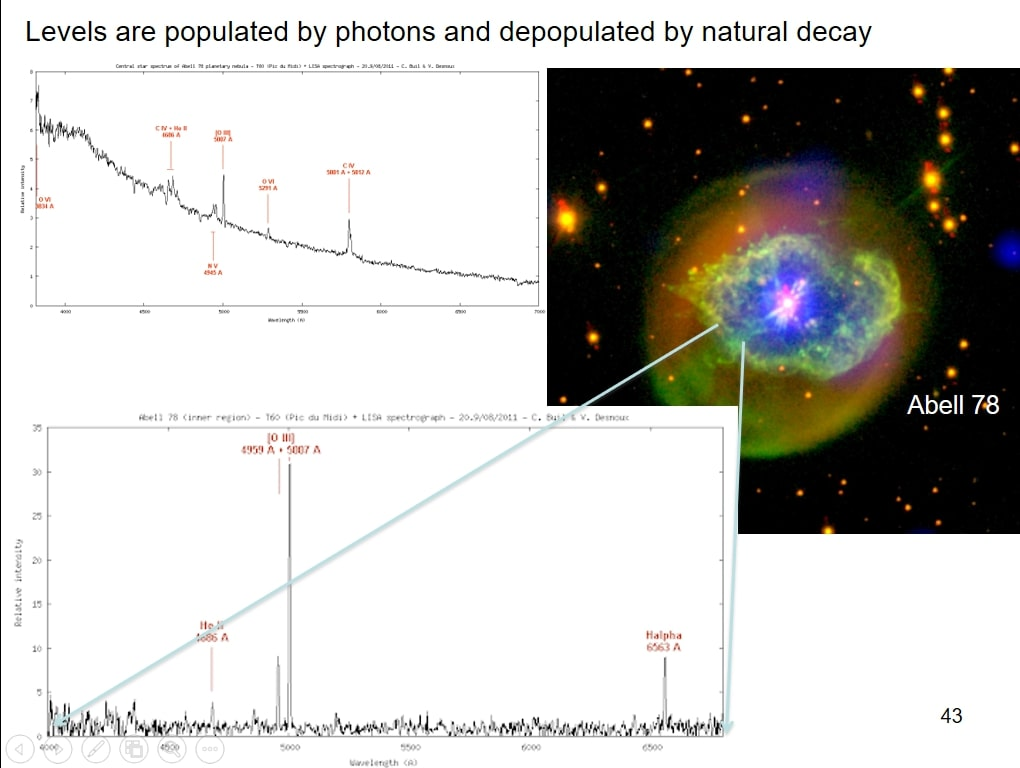
\includegraphics[width=9cm]{abell.jpg}
  %\caption{Nebulosa planetaria Abell 78 e relativi spettri}
  \label{fig:Abell}
\end{figure}

\subsubsection{Curve di crescita}

Il centro di una riga in assorbimento o in emissione corrisponde in genere ad una transizione atomica ben precisa e misurabile in laboratorio. Per descrivere in maggior dettaglio una riga si deve definire la sua profondità, cioè l'assorbimento al massimo, e la sua larghezza. Una possibile definizione di quest'ultima è la cosiddetta Full Width at Half Maximum, o FWHM, che dà la larghezza totale della riga a metà del massimo di assorbimento o di emissione.

Per quantificare l'intensità spettrale di una riga si utilizza la definizione di \textbf{larghezza equivalente} di una riga spettrale

$$W_{\lambda}=\int_{0}^{\infty} A_{\lambda} \, d{\lambda}
\quad \text{con} \quad
A_{\lambda}=\frac{F_c - F_{\lambda}}{F_c}$$

dove $A$ è la profondità di riga, $F_c$ è il valore del flusso al continuo e $F$ è il flusso relativo alla riga. Tale integrale è equivalente all'area di un rettangolo di altezza unitaria e base pari alla larghezza di quella riga. Ecco perché si chiama larghezza equivalente. Solitamente si misurano in m\AA.

\begin{figure}[H]
  \centering
  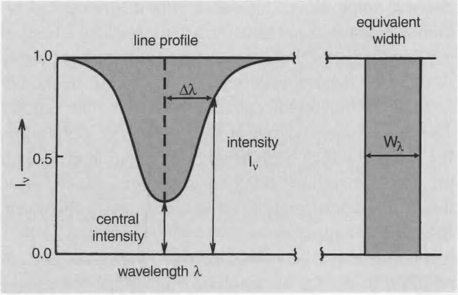
\includegraphics[width=6cm]{immagini/equivalent_width.png}
\end{figure}

Vediamo adesso come cambia l'intensità di una riga spettrale per effetto dell'abbondanza di un elemento.

\begin{figure}[H]
  \centering
  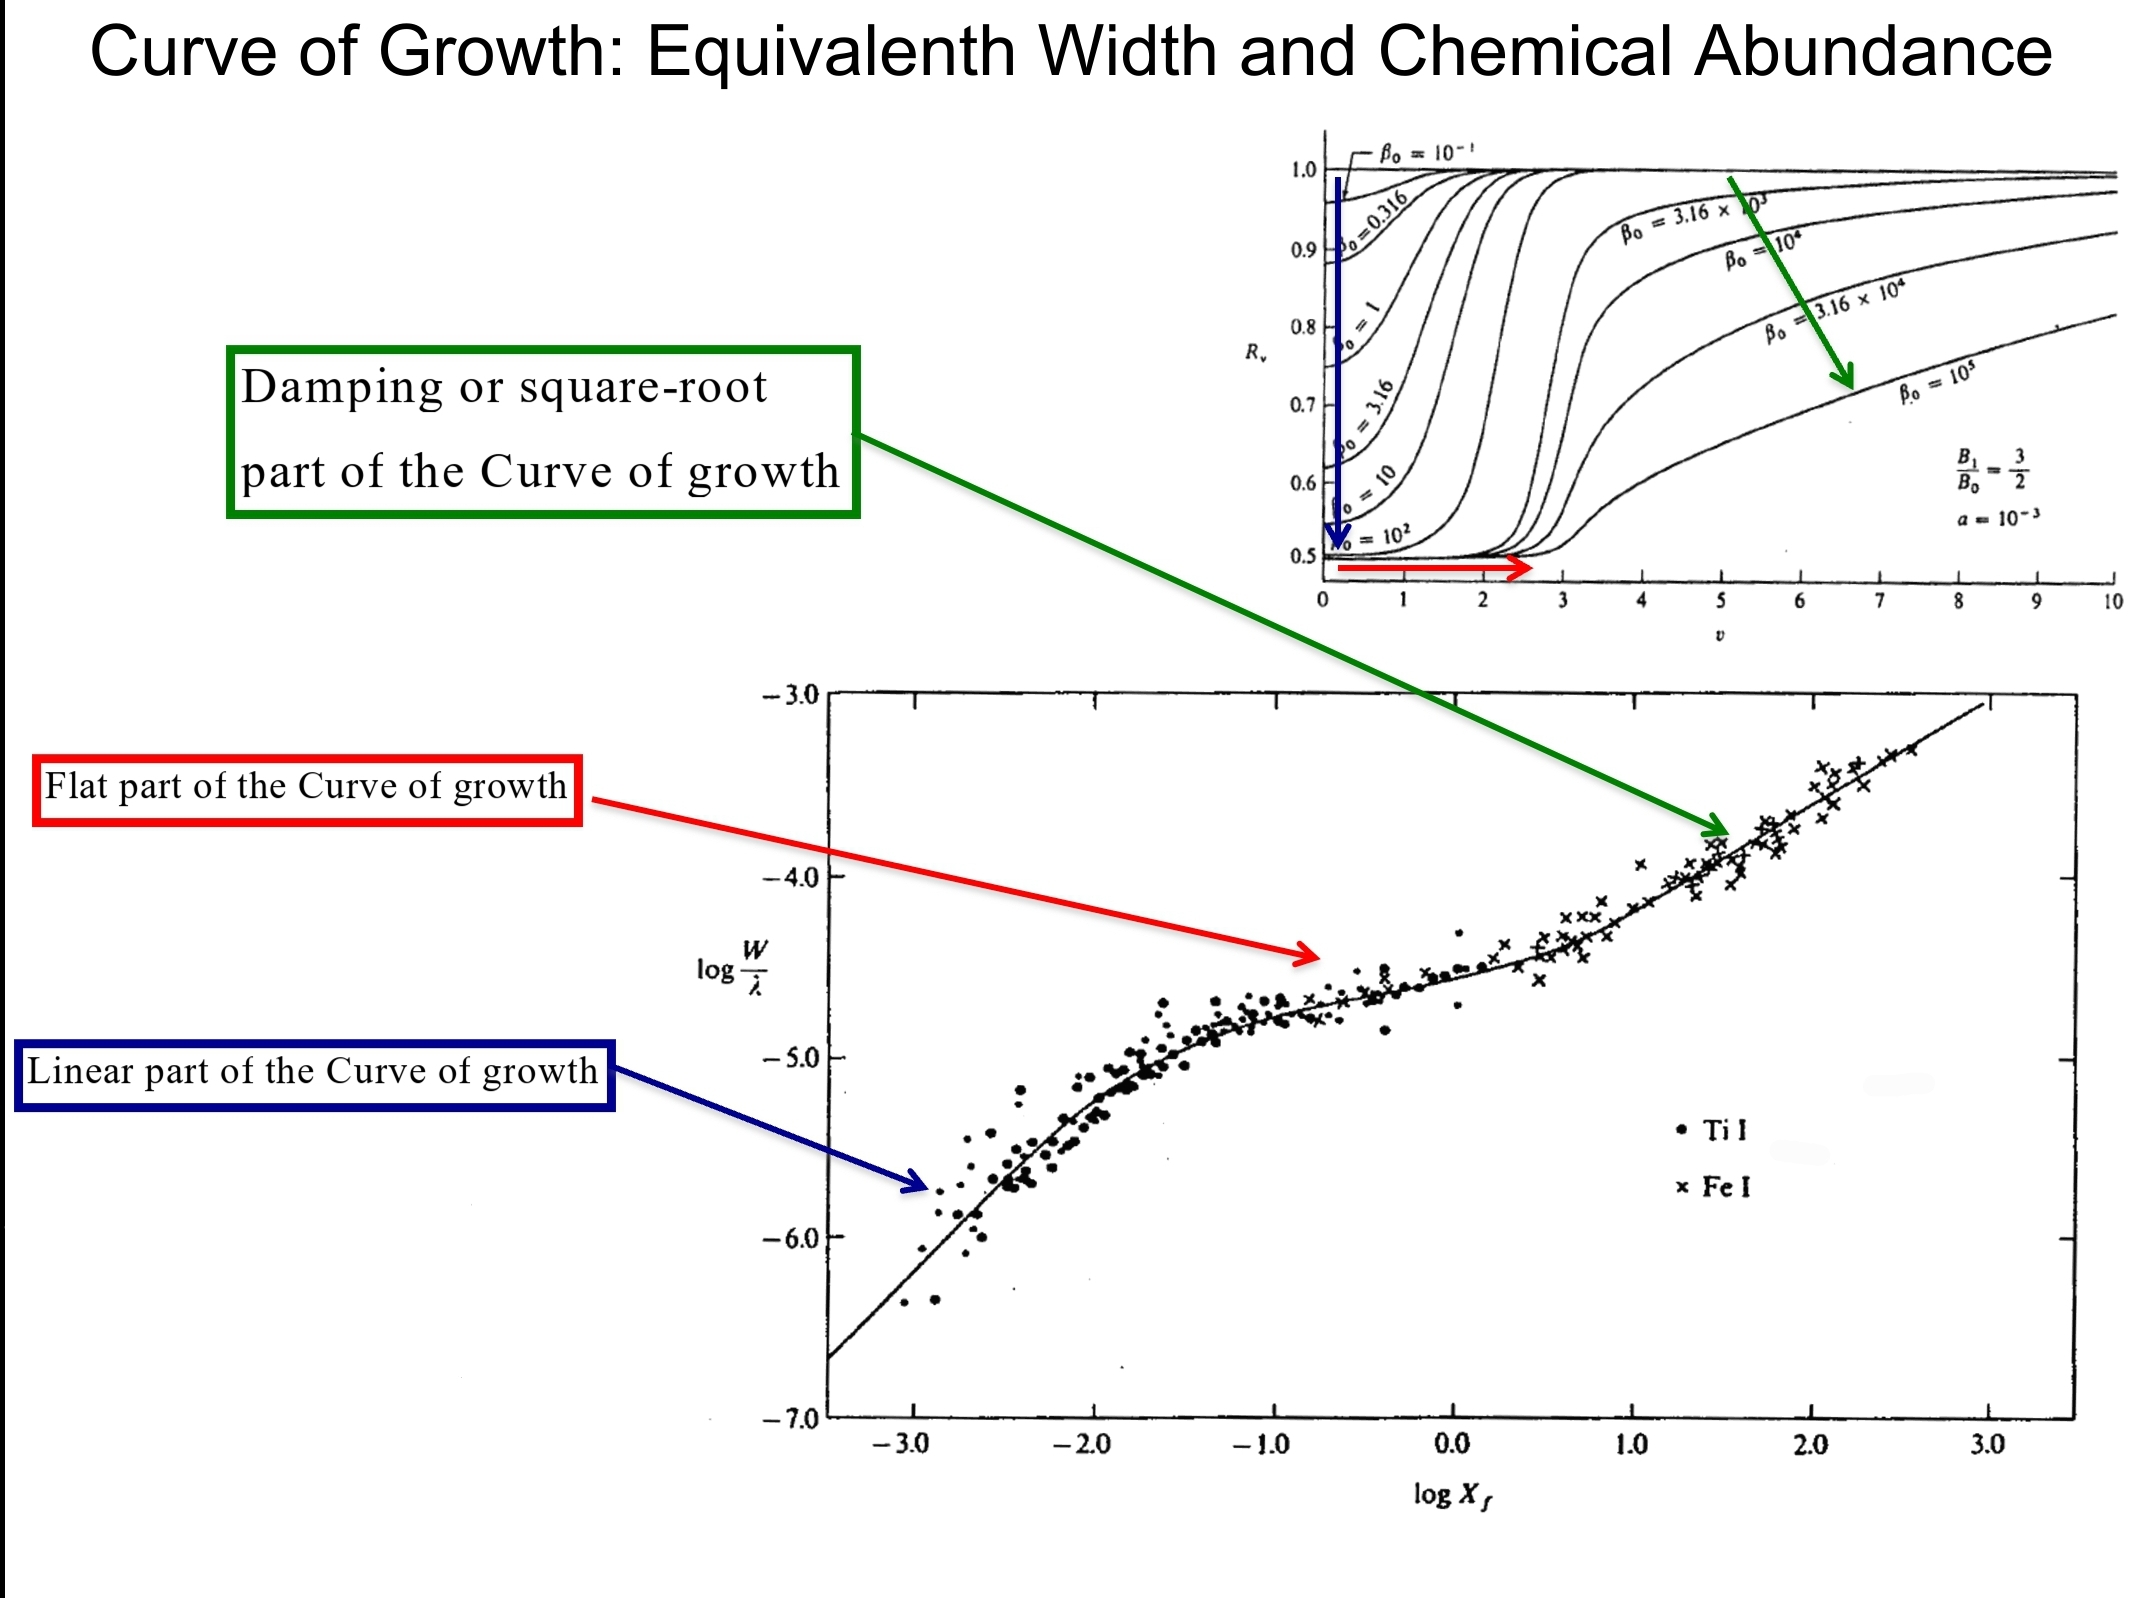
\includegraphics[width=9cm]{curva.jpg}
\end{figure}

Tutti abbiamo l'idea istintiva che più è abbondante un elemento, più grande sarà una riga (o in assorbimento o in emissione). Ricordiamo che la larghezza equivalente è la larghezza di un rettangolo che ha area pari all'ampiezza della riga. Nella curva in figura, normalmente nota come curva di crescita, risultato di molti calcoli e osservazioni, si riporta la larghezza equivalente di una riga spettrale in funzione del numero di atomi coinvolti nella riga. Finché gli assorbitori sono pochi, al loro aumentare si osserva una crescita lineare della larghezza equivalente: questo è intuitivo perché, come detto precedentemente, il coefficiente di estinzione, nel caso in cui la sezione d'urto è molto più piccola della distanza media delle particelle, è proporzionale alla sezione d'urto e il coefficiente di proporzionalità è proprio il numero di assorbitori. Dopo la parte lineare della curva di crescita, si ha una parte in cui si va in una sorta di saturazione: non ha importanza se si aumenta il numero di assorbitori, la quantità di fotoni che passa è comunque la stessa e quindi la larghezza equivalente non cresce di moltissimo. Quando, infine, il numero di assorbitori diventa enorme, la larghezza equivalente cresce con la radice quadrata del numero di assorbitori; in tale regime è dominante il contributo dell'allargamento collisionale alle ali della riga.



\E chiaro che questo andamento dipende dalle abbondanze degli elementi. La composizione chimica che conosciamo noi nasce dallo studio dei meteoriti. La maggior parte degli atomi è costituita da Idrogeno\footnote{ovviamente non si ci si può riferire al numero totale di atomi di Idrogeno in una stella, ma si ragiona in percentuale.}, che costituisce circa il 90\% degli elementi, poi abbiamo in minori quantità Elio (10\%). Tutto il resto degli elementi vengono definiti "tracce" (i più abbondanti tra questi sono Ossigeno, Carbonio e Azoto), tanto che i valori relativi all'abbondanza si rappresentano in scala logaritmica.

